% Preamble
\documentclass[11pt]{article}

% Packages
\usepackage{amsmath}
\usepackage{amssymb}
\usepackage{tikz}
\usetikzlibrary{arrows,arrows.meta,positioning,calc,petri}
\usepackage{adjustbox}
\usepackage{enumitem}
\usepackage{listings}
\usepackage[ruled,vlined]{algorithm2e}
\SetKwRepeat{Do}{do}{until}%
\newtheorem{theorem}{Theorem}

% Document
\begin{document}

    \section*{Rule L: Dominated Transition}\label{sec:rule_l}
    Rule L removes transitions that have the same effect as another transition, but with more preconditions.
    Since both transitions lead to the same state, we can therefore remove the one
    with the higher preconditions and use the other instead.
    See the formal description in Figure~\ref{fig:rule_l}.

    \begin{figure}[h!]
        \centering
        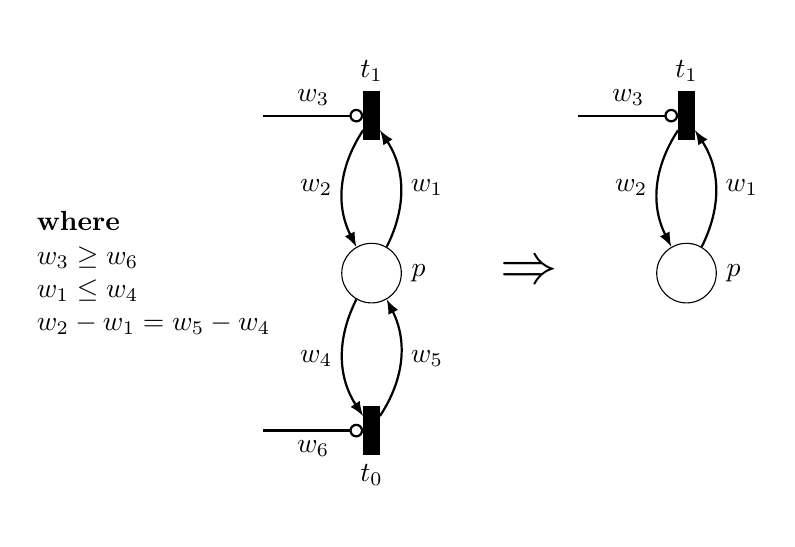
\begin{tikzpicture}
            % Left side places
            \node[place, label=right:$p$] (place1) at (0,0) {};

            % Left side transition
            \node[transition,minimum height=6mm,minimum width=2mm,fill=black,label=above:$t_1$] (lTrans1) at (0,2) {};
            \node[transition,minimum height=6mm,minimum width=2mm,fill=black,label=below:$t_0$] (lTrans2) at (0,-2) {};

            % Left side invisible nodes
            \node (negIn1) at (-1.5,2) {};
            \node (negOut1) at (1,3) {};
            \node (remIn1) at (-1.5,-2) {};
            \node (remOut1) at (1,-3) {};

            % Left side arcs between transitions and nodes
            \draw[-latex,thick] (lTrans1) edge[bend right] node[left] {$w_2$} (place1);
            \draw[-latex,thick] (place1) edge[bend right] node[right] {$w_1$} (lTrans1);
            \draw[-latex,thick] (lTrans2) edge[bend right] node[right] {$w_5$} (place1);
            \draw[-latex,thick] (place1) edge[bend right] node[left] {$w_4$} (lTrans2);

            % Left side arcs to/from invisible nodes
            \draw[-{Circle[open]},thick] (negIn1) -- node[above] {$w_3$} (lTrans1);
            \draw[-{Circle[open]},thick]  (remIn1) -- node[below] {$w_6$} (lTrans2);

            % ================== Middle arrow ==================
            \node (arrow) at (2,0) {\huge$\Rightarrow$};
            \node[text width=3.5cm] at (-2.5,0) {\textbf{where }\\$w_3\geq w_6$\\$w_1\leq w_4$\\$w_2-w_1= w_5-w_4$};
            % ==================================================

            % Right side places
            \node[place, label=right:$p$] (place2) at (4,0) {};

            % Right side transitions
            \node[transition,minimum height=6mm,minimum width=2mm,fill=black,label=above:$t_1$] (rTrans1) at (4,2) {};

            % Right side invisible nodes
            \node (negIn2) at (2.5,2) {};

            % Right side arcs between places and transition
            \draw[-latex,thick] (rTrans1) edge[bend right] node[left] {$w_2$} (place2);
            \draw[-latex,thick] (place2) edge[bend right] node[right] {$w_1$} (rTrans1);

            \draw[-{Circle[open]},thick]  (negIn2) -- node[above] {$w_3$} (rTrans1);


        \end{tikzpicture}
        \vspace{5mm}
        \begin{adjustbox}{center}
            \begin{tabular}{|p{55mm}|p{45mm}|} \hline
            Precondition & Update \\ \hline
            Fix transition $t_1$ and $t_0$ s.t.:
            \begin{itemize}[leftmargin=10mm]
                \item[L1)] $I(t_1)\geq I(t_0)$
                \item[L2)] $\boxminus(t_1)\leq \boxminus(t_0)$
                \item[L3)] $E(t_1)=E(t_0)$
            \end{itemize}
            &
            \begin{itemize}[leftmargin=10mm]
                \item[UL1)] Remove $t_0$
            \end{itemize} \\ \hline
            \end{tabular}
        \end{adjustbox}
        \caption{Rule L: Dominated Transition}
        \label{fig:rule_l}
    \end{figure}

    \begin{theorem}
        Rule~L in Figure~\ref{fig:rule_l} is correct for CTL*.
    \end{theorem}

\end{document}
